%--------------------------------------------CAPA DE TECNOLOGIA ------------------------------------------------------%


\subsection{Capa de tecnología}

Los elementos de la capa tecnológica se utilizan normalmente para modelar la arquitectura tecnológica de la empresa, describiendo \textbf{la estructura y el comportamiento de la infraestructura tecnológica de la empresa.}
La Tabla \ref{tab:Tabla de la capa de tecnología} ofrece una descripción general de los elementos de la capa tecnológica, con sus definiciones.\cite{archimate} 
\begin{longtable}{|p{0.15\linewidth}|p{0.45\linewidth}|p{0.4\linewidth} |}
    \caption{Tabla de la capa de tecnología}
    \\
    \hline
    \rowcolor[HTML]{AFC5F6} 
    \textbf{Elemento} & \textbf{Descripción} & \textbf{Notación} \\
    \hline
    \endhead
    \hline
    \multicolumn{3}{r}{\textit{Continúa en la siguiente página}} \\
    \endfoot
    \hline
    \endlastfoot
    \label{tab:Tabla de la capa de tecnología}
    %Contenido 1 &
    %\lipsum[1] &
    %Datos A1
    %& Datos B1
    %\\
    %\hline



    Nodo
    &
    Representa un recurso físico o computacional 
        que aloja, manipula o interactúa con otros 
        recursos físicos o computacionales.
    &
\begin{center}
    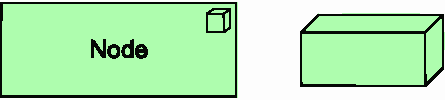
\includegraphics[width=0.8\linewidth]{imgs/capa_tecnologia/Node.pdf}
\end{center} 
    \\ \hline



    Dispositivo
    &
    Representa un recurso físico de TI sobre el cual 
    se pueden almacenar o implementar software y 
    artefactos del sistema para su ejecución.
    &
\begin{center}
    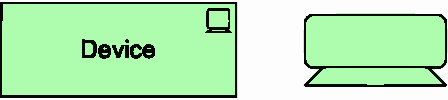
\includegraphics[width=0.8\linewidth]{imgs/capa_tecnologia/Device.pdf}
\end{center} 
    \\ \hline



    Software del sistema 
    &
    Representa software que proporciona o 
    contribuye a un entorno para almacenar, 
    ejecutar y utilizar software o datos 
    implementados en él.
    &
\begin{center}
    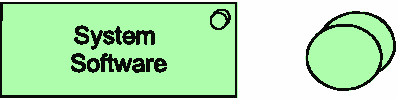
\includegraphics[width=0.8\linewidth]{imgs/capa_tecnologia/System software.pdf}
\end{center} 
    \\ \hline



    Colaboración tecnológica
    &
    Representa un agregado de dos o más elementos 
        de estructura activa interna de tecnología que 
        trabajan juntos para realizar un 
        comportamiento tecnológico colectivo.
    &
\begin{center}
    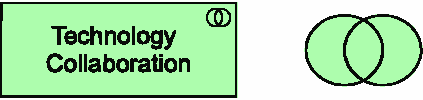
\includegraphics[width=0.8\linewidth]{imgs/capa_tecnologia/Technology collaboration.pdf}
\end{center} 
    \\ \hline

    Interfaz tecnológica
    &
    Representa un punto de acceso donde se puede 
    acceder a los servicios tecnológicos ofrecidos por 
    una estructura activa interna de tecnología.
    &
\begin{center}
    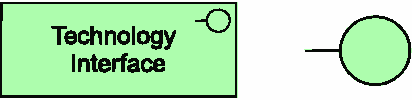
\includegraphics[width=0.8\linewidth]{imgs/capa_tecnologia/Technology interface.pdf}
\end{center} 
    \\ \hline

    Camino
    &
    Representa un vínculo entre dos o más 
        elementos tecnológicos de estructura activa 
        interna, a través del cual estos elementos 
        pueden intercambiar datos, energía o material.
    &
\begin{center}
    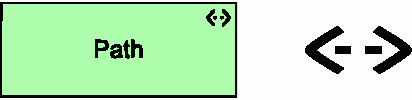
\includegraphics[width=0.8\linewidth]{imgs/capa_tecnologia/Path.pdf}
\end{center} 
    \\ \hline

    Red de comunicación
    &
    Representa un conjunto de estructuras que 
    conectan dispositivos o software del sistema 
    para la transmisión, enrutamiento y recepción 
    de datos.
    &
\begin{center}
    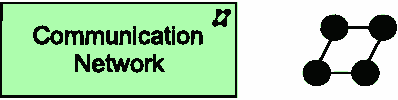
\includegraphics[width=0.8\linewidth]{imgs/capa_tecnologia/Communication network.pdf}
\end{center} 
    \\ \hline

    Función tecnológica
    &
    Representa una colección de comportamientos 
        tecnológicos que puede realizar un elemento de 
        estructura activa interna de tecnología.
    &
\begin{center}
    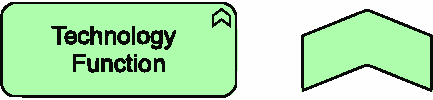
\includegraphics[width=0.8\linewidth]{imgs/capa_tecnologia/Technology function.pdf}
\end{center} 
    \\ \hline

    Proceso tecnológico
    &
    Representa una secuencia de comportamientos 
    tecnológicos que logra un resultado específico.
    &
\begin{center}
    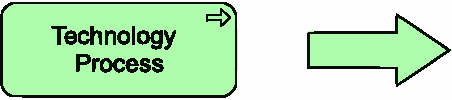
\includegraphics[width=0.8\linewidth]{imgs/capa_tecnologia/Technology process.pdf}
\end{center} 
    \\ \hline

    Interacción 
    tecnológica
    &
    Representa una unidad de comportamiento 
        tecnológico colectivo realizado por (una 
        colaboración de) dos o más elementos 
        tecnológicos internos de la estructura activa.
    &
\begin{center}
    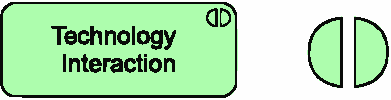
\includegraphics[width=0.8\linewidth]{imgs/capa_tecnologia/Technology interaction.pdf}
\end{center} 
    \\ \hline

    Evento Tecnológico
    &
    Representa un cambio de estado de la 
    tecnología.
    &
\begin{center}
    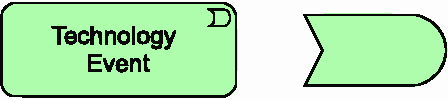
\includegraphics[width=0.8\linewidth]{imgs/capa_tecnologia/Technology event.pdf}
\end{center} 
    \\ \hline

    Servicio de tecnología
    &
    Representa un comportamiento de tecnología 
    expuesta explícitamente definido.
    &
\begin{center}
    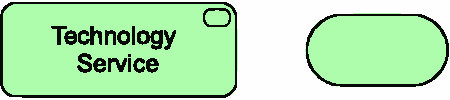
\includegraphics[width=0.8\linewidth]{imgs/capa_tecnologia/Technology service.pdf}
\end{center} 
    \\ \hline

    Artefacto
    &
    Representa un dato que se utiliza o se produce 
        en un proceso de desarrollo de software, o 
        mediante la implementación y operación de un 
        sistema de TI.
    &
\begin{center}
    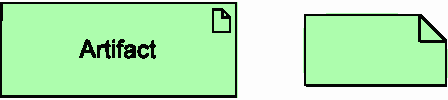
\includegraphics[width=0.8\linewidth]{imgs/capa_tecnologia/Artifact.pdf}
\end{center} 
    \\ \hline

\end{longtable}